% Main file for the GREIT Algorithm
% $Id$
\documentclass[12pt,draft]{iopart}
\usepackage{graphicx}
 \usepackage{amssymb}
 \usepackage{amsbsy}
\newcommand{\vB}{\mbox{$\mathbf{v}$}}
\newcommand{\xB}{\mbox{$\mathbf{x}$}}
\newcommand{\xH}{\mbox{$\mathbf{\hat x}$}}
\newcommand{\xT}{\mbox{$\mathbf{\tilde x}$}}
\newcommand{\XT}{\mbox{$\mathbf{\tilde X}$}}
\newcommand{\nB}{\mbox{$\mathbf{n}$}}
\newcommand{\yB}{\mbox{$\mathbf{y}$}}
\newcommand{\wB}{\mbox{$\mathbf{w}$}}
\newcommand{\AB}{\mbox{$\mathbf{A}$}}
\newcommand{\BB}{\mbox{$\mathbf{B}$}}
\newcommand{\RB}{\mbox{$\mathbf{R}$}}
\newcommand{\IB}{\mbox{$\mathbf{I}$}}
\newcommand{\JB}{\mbox{$\mathbf{J}$}}
\renewcommand{\PB}{\mbox{$\mathbf{P}$}}
\newcommand{\VB}{\mbox{$\mathbf{V}$}}
\newcommand{\WB}{\mbox{$\mathbf{W}$}}
\newcommand{\XB}{\mbox{$\mathbf{X}$}}
\newcommand{\YB}{\mbox{$\mathbf{Y}$}}
% Use boldsymbol when using amssymb
 \newcommand{\SG}{\mbox{${\boldsymbol \Sigma}$}}
 \newcommand{\TG}{\mbox{${\boldsymbol \Theta}$}}
 \newcommand{\sG}{\mbox{${\boldsymbol \sigma}$}}
%\newcommand{\SG}{\mbox{${\mathbf \Sigma}$}}
%\newcommand{\TG}{\mbox{${\mathbf \Theta}$}}
%\newcommand{\sG}{\mbox{${\mathbf \sigma}$}}
\newcommand{\SNR}{\mbox{\small $\mathrm{SNR }$}}
\newcommand{\NF}{\mbox{\small $\mathrm{NF }$}}
\newcommand{\EIT}{\mbox{\small $\mathit{EIT }$}}
\begin{document}

\title[FEM variability and EIT images]{%
 Compensating for EIT image reconstruction errors due to 
   FEM variability 
}
%{\small \tt DRAFT: $Date$}

\author{Andy Adler$^{1}$,
        William R B Lionheart$^{2}$,
       }

\address{ $^{1}$Systems and Computer Engineering,
                Carleton University, Ottawa, Canada}
\address{$^{13}$School of Mathematics, University of Manchester, UK}



\begin{abstract}
Electrical Impedance Tomography (EIT)
\end{abstract}

\noindent{\it Keywords\/}:
Electrical Impedance Tomography,
Image Reconstruction,
Finite Element Models

\section{Introduction}
In this paper, we describe the image reconstruction artefacts
which occur in electrical impedance tomography (EIT) images
due to limitations in the finite element models, and show
an algorithmic approach to limit such effects.
%
EIT is a technology designed to measure conductivity
changes within a body using electrical stimulations and
measurements at electrodes on the body surface. Typically,
a set of sinusoidal current patterns are sequentially applied to
the electrodes and the resulting voltages measured. This
set of measurements constitues an EIT data frame, from which
and images may then by reconstructed of the body's internal impedance
distribution (absolute imaging) or the change in impedance distrubution
between two data frames (time difference imaging). EIT thus has
the advantage of providing tomographic information about a body
from measurements from equipment which is non-invasive, minimally
cumbersome and potentially inexpensive (REFS).
 
Reconstruction of EIT images requires solving an ill-conditioned
or ill-posed inverse problem (REFS).
 EIT is ill-posed because we typically
seek to reconstruct onto much larger image than the number of
independent measurements.
 The ill-conditioning is
due to the physics of current propagation; most current stays
close to the source electrodes on the body surface, while only
a much smaller fraction penetrates the interior, which is typically
the focus of interest.
One further consequence of the current propagation is the extreme
sensitivity to the shape of the body surface and exact electrode
placements and properties (REFS). One technique to deal with
shape and electrode uncertainties is the use of time difference
imaging, in which is less sensitive to shape uncertainties which do
not change between data frames (Adler \etal, 1996).

The earliest approaches to EIT image reconstruction were
based on 2D circular approximations of the thorax 
(Barber and Brown, 1988; Seagar and Bates, 1985). However, since
such analytical models cannot describe electrical propagation
in realistic body shapes, finite element models begun to be
used (Murai and Kagawa, 1985; Yorkey \etal 1987). Over the
last two decades, the FEM has become the most popular approach
to model EIT current distrubutions. Other numerical models,
such as those based on finite differences (Yang and Patterson,
2007) have been used, but are less popular, primarily
because FEM mesh elements can be easily refined in regions
of high electric field, typically near to electrodes.

While the FEM literature is rich in terms of variety of
model structure, most EIT research has used the simplest
FEM implementations. Elements are chosen to be simplices
shapes (trianges in 2D and tetrahedrons in 3D) and conductivity
is modelled as piecewise constant (so that changes in conductivity
occur only at element boundaries). Such choices are reasonable:
all FEM meshing packages provide good support for simplex
elements, and anatomically realistic conductivity changes
do occur abruptly at organ boundaries. 

Additionally, two further FEM approximations are typically made.
First, first order elements are used. This means that voltages
across each element interpolate linearly between nodes at
the vertices. Physically, such elements may be modelled by a
resistor network (Murai and Kagawa, 1985). This certainly
makes such a FEM easier to understand and may be used as
the basis for a physical resistor network model of the medium
(Gagnon \etal 2008). On the other hand, FEM model errors decrease
linearly with element size for first order FEMs, while the
rate of error decrease is larger for higher order models.
Next, the conductivity is assumed to be isotropic. While many
tissues are (macroscopically) anisotropic, it is difficult to
measure these properties and few published values exist. Thus,
it can make sense to simply ignore anisotropy in a model.
On the other hand, the anisotropic effects can be included
into the FEM fairly straightforwardly (Abascal \etal 2007, 
Abascal \etal 2008).

Image reconstruction in EIT



\section{Forward models}

\subsection{Finite Element Models}

FEMs are generate using the Netgen (Sch\"oberl, 1997) mesh
generation software, which builds FEM models to arbitrary
solid geometry constructions. An interface to Netgen is
provided by EIDORS (Adler \etal, 2006) in which electrodes
are specified by the intersection of the main body volume
and cylindrical shapes normal to the boundary. Mesh refinement
is implemented by specifying the maximum element size permissible
in each electrode and body volumes. In order to include shapes
into the meshed volume, a sphere within the body volume 
is defined into the solid geometry model.

\subsection{Analytic Model}


\begin{figure}[tbh]
\begin{center}
 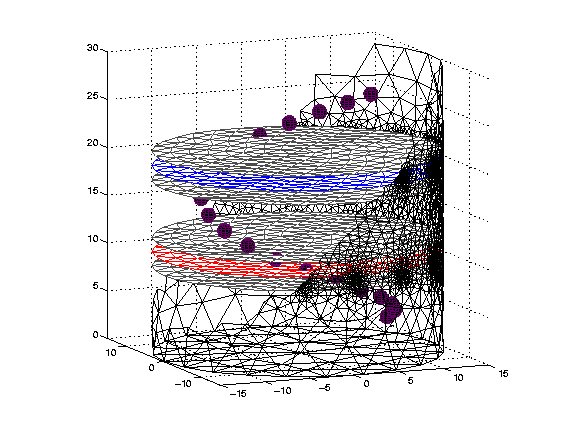
\includegraphics[width= 0.45\textwidth, bb=0 0 466 278]{../../tutorial/dual_model/centre_slice02a.png}
\caption{ \label{fig:dual_model}
\small
Netgen model of a $2\times 16$ electrode tank. The positions of the simulated
conductive target moving in a helical path are shown in purple. The
3D fine model is shown (cropped). The upper (blue) and lower (red)
layers corresponding to the geometry of the coarse model are shown. The
$z$-direction limits of the coarse model are shown in grey.
}
\end{center}

\end{figure}

\section{Image Reconstruction}

\begin{figure}[tbh]
\begin{center}
 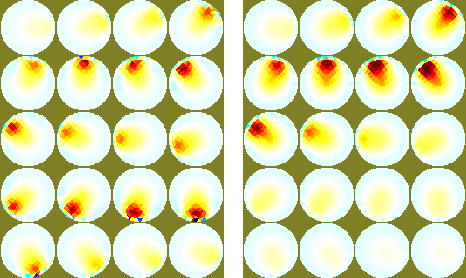
\includegraphics[width= 0.45\textwidth, bb=0 0 588 508]{../paper-EIT2008/figs/centre_slice04a_crop.png}
\caption{ \label{fig:dual_model_reconst}
\small
Reconstructed images of a target moving in a helical pattern using
difference reconstruction models.
{\em Left} reconstruction model with  $z_{depth}=\infty$
{\em Right} reconstruction model with $z_{depth}= 0.1\times \mbox{scale}$
at lower position in Fig.~\ref{fig:dual_model}
}
\end{center}
\vspace{-0.5cm}
\end{figure}

\subsection{Dual Model solvers}


A dual reconstruction model uses a high density (fine)
FEM to implement the forward solution (voltages
at electrodes), and a low density (coarse) mesh
(not necessarily FEM based) for the inverse
solution. For example, a dual model may be used to 
represent the conductivity change in a layer
of a 3D plane (Fig.~\ref{fig:dual_model}).
Given a forward model, $F$,
which calculates a voltage measurement vector, $\vB$, from
a forward (fine) model conductivity element vector, $\sG_f$, we
have $\vB = F( \sG_f )$. The reconstruction (coarse)
model is defined on square elements $\sG_r$ related by
a coarse to fine projection matrix $\PB$, where $\sG_f = \PB \sG_r$.

This is implemented in EIDORS as follows. For each
inverse model, represented as part of the {\tt inv\_model}
structure (Fig.~\ref{fig:invmdl}),
there are two {\tt fwd\_model} structures:
1) the refined forward model {\tt fwd\_model}, and
2) the reconstruction model {\tt rec\_model}. 
Within each forward model structure is a matrix field
{\tt coarse2fine} which is a sparse encoding of $\PB$.
Each element $[\PB]_{i,j}$ represents the fraction of
fine element $i$ enclosed within coarse element $j$.

The Jacobian matrix may be defined for the coarse
($\JB_r$) and fine ($\JB_f$) models as follows:
\begin{equation}
\vB = \JB_f \sG_f 
    = \JB_f \PB \sG_r
    = \JB_r     \sG_r
\end{equation}
and thus $\JB_r = \JB_f \PB$. Since the matrix
$\JB_f$ is very large, EIDORS will not calculate it
directly. Instead, an efficient algorithm calculates
each column of $\JB_r$ using
\begin{equation}
\big[ \JB_c \big]_{i,j} =
\big[ \JB_f \PB \big]_{i,j} =
\sum_k \frac{\partial [ \vB ]_i }
            {\partial [ \sG_f ]_k } [\PB]_{k,j}
= \frac{\partial [ \vB ]_i }
       {\partial [ \sG_c ]_j }
\end{equation}
where the last expression is implemented in terms
of the FEM system matrix using the adjoint field method.

The need for a matrix $\PB$ on the {\tt rec\_model} is
due to the limits of the first order FEM representation.
If the regions in the reconstruction model are not
triangular, then each region is constructed from triangular
regions and the parametrization represented in $\PB$.

\begin{figure}[tbh]
\begin{center}
 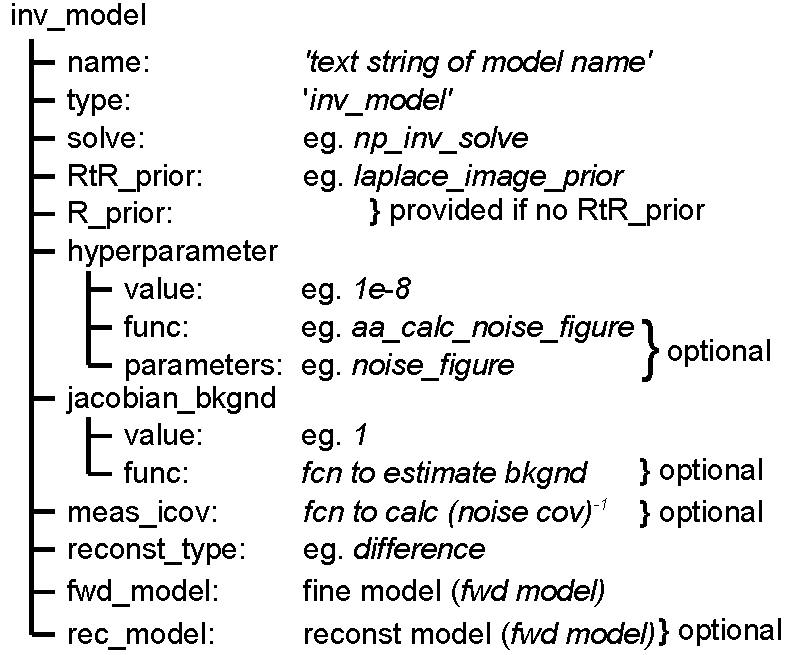
\includegraphics[width= 0.40\textwidth,bb=0 0 788 655]{../paper-EIT2008/figs/inv_model.png}
\caption{ \label{fig:invmdl}
\small
Layout of the EIDORS {\tt inv\_model} object
}
\end{center}
\vspace{-0.5cm}
\end{figure}

Dual meshes may be used in several applications:
\begin{list}{$\circ$} %{\textbullet}
  {\leftmargin=1.0em \itemindent=-0.0em
    \topsep=0.0\baselineskip
    \itemsep=-0.4\baselineskip}
\item
   Corresponding meshes: where 
   coarse elements completely contain fine ones but do not
   cross elements.
\item
   Nodal Solvers: in which the reconstruction parameterizes
   the conductivity on each node\cite{graham2006}.
\item
   $2\frac{1}{2}$D Solvers: in which the $z$-dimension of the
     3D fine model is projected onto a 2D reconstruction model.
     This technique is widely used in geophysical appications.
\item
   Constraining Reconstruction Parameters:
      this is useful for example to have one parameter
      for out of plane conductivity (a region of low sensitivity),
      which may prevent the algorithm from ``pushing" artefacts there.
\item
   Solving to a Square Pixel Grid: this is useful because the
       reconstructed image is typically mapped to pixels, and
       will often show artefacts based on the shapes of the elements.
       A rasterized reconstruction grid will prevent such
       artefacts, and allow more natural communication of the
       underlying system resolution (via the pixel size).
\end{list}


%Dual meshes have been used by many EIT groups
%\\
%- Oxford Brookes used an interpolation method on two meshes since the early code in the Fortran code Recon started by Lionheart and continued by Kevin Paulson at Brookes. The approach used a mesh correspondence array. 
%\\
%- Later on the Dartmouth group also used the idea; paper by the
%   similarly named Keith Paulsen (ref).
%\\
%- Marko Vauhkonen use two meshes in the original 2D EIDORS.
%\\
%- UCL optimal tomography group uses it for TOAST.
%



\References % Harvard style references
\item[]
Adler A and Guardo R 1996 Electrical impedance tomography:
regularized imaging and contrast detection {\em IEEE Trans. Med.
Imaging} {\bf 15} 170-179

\item[]
Adler A, Guardo R and Berthiaume Y 1996 Impedance imaging of lung
ventilation: Do we need to account for chest expansion? {\em IEEE
Trans. Biomed. Eng.} {\bf 43}(4) 414-20


\item[]
Adler A and Lionheart W R B 2006
Uses and abuses of EIDORS: An extensible software base for EIT
{\em Physiol Meas}
27 S25--S42

\item[]
Abascal J P J, Arridge S R, Lionheart W R B, Bayford R H, Holder D S  2007
Validation of a finite element solution for electrical impedance tomography in an anisotropic medium
{\em Conf. ICEBI} Graz, Austria.
IFMBE Proc. 17:372--375

\item[]
Abascal J P J, Arridge S R, Atkinson D, Horesh R, Fabrizi L, Horesh L, Bayford R H, Holder D S  2008
Use of anisotropic modelling in electrical impedance tomography; Description of method and preliminary assessment of utility in imaging brain function in the adult human head
{\em NeuroImage} 43:258--268


%\item[]
%Barber D C
%Brown B H
%Freeston I L, 1983
%Imaging spatial distributions of resistivity using applied potential tomography
%{\em Electronics Letters}
%19 933--935
%

\item[]
Barber D C and Brown B H 1984
Applied potential tomography
{\em J Phys E: Sci Instrum}
 17 723--733

\item[]
Barber D C and Brown B H 1988 Errors in reconstruction of
resistivity images using a linear reconstruction technique {\em
Clin. Phys. Physiol. Meas.} 
9(suppl. A) 101--4

\item[]
Barber D C 1989
A review of image reconstruction techniques for electrical
 impedance tomography
{\em Med Phys}
16 162--169


\item[]
Brown B W 2003
Electrical impedance tomography (EIT): a review
{\em J Medical Eng. \& Technology}
27 97--108


\item[]
Cheney M, Isaacson D, Newell J C, Simske S and Goble J C 1990
NOSER: an algorithm for solving the inverse conductivity problem
{\em Int J Imaging Syst Technol} 
2 66--75

\item[]
Cheng KS, Newell JC, Gisser DG, 1989
Electrode Models for Electric Current Computed Tomography
{\em IEEE Trans in Biomedical Eng}
36 918--924

\item[]
Gagnon H, Hartinger A E, Adler A, Guardo R 2008
A phantom for assessing the performance of EIT systems
{\em Proc.\ Conf.\ EIT}, Hannover, NH, USA


\item[]
G\'omez-Laberge C Adler A 2008
Direct EIT Jacobian calculations for conductivity change and electrode movement
{\em Physiol Meas}
29 S89--S99


\item[]
Hahn G Just A Dittmar J  Hellige G 2008
Systematic errors of EIT systems determined by easily-scalable
 resistive phantoms
{\em Physiol Meas}
 29 S163--S172
 
\item[]
Lionheart W R B 2004
EIT reconstruction algorithms: pitfalls, challenges
and recent developments
{\em Physiol Meas}
25 125--142

\item[]
Murai T, Kagawa Y 1985
Electrical impedance computed tomography based on finite element model
{\em IEEE T Biomed Eng} 32:177-184

\item[]
Oh S, Tang T, Sadleir R 2007
Quantitative analysis of shape change in Electrical Impedance Tomography (EIT)
in {\em IFMBE Proceedings}
17 424--427

\item[]
Polydorides N and Lionheart W R B 2002 A Matlab toolkit for
three-dimensional electrical impedance tomography: A contribution
to the Electrical Impedance and Diffuse Optical Reconstruction
Software project {\em Meas Sci Technol} {\bf 13} 1871-83

\item[]
Sch\"oberl J 1997
NETGEN: An advancing front 2D/3D-mesh generator based on abstract rules
{\em Computing and Visualization in Science}
1 41--52 

\item[]
Seagar A D Bates R H T 1985
Full-wave computed tomography. Part 4: Low-frequency electric current CT
{\em IEE Proceedings A} 132: 455--466

\item[]
Soleimani M, G\'omez-Laberge C and Adler A 2006 Imaging of
conductivity changes and electrode movement in EIT
{\em Physiol Meas} {\bf 27}
S103--S13

\item[]
Shaw G R  Goussard  Y Guardo R  1993 
Linearization of the forward problem in electrical impedance tomography
{\em Proc. Conf. IEEE EMBS} 82-83

\item[]
Tizzard A Horesh L Yerworth R J Holder D S Bayford R H 2005
Generating accurate finite element meshes for the forward
model of the human head in EIT
{\em Physiol Meas}
 26 S251--61 

\item[]
Yorkey T J, Webster J G and Tompkins W J 1987
Comparing reconstruction algorithms for electrical
impedance tomography
{\em IEEE Trans. Biomed. Eng}
34 843--52

\item[]
Yang F  Patterson R 2007
The contribution of the lungs to thoracic impedance
measurements: a simulation study based on a high
resolution finite difference model
{\em Physiol. Meas.}
28 S153--S163

\endrefs

\end{document}
